% This is "sig-alternate.tex" V2.1 April 2013
% This file should be compiled with V2.5 of "sig-alternate.cls" May 2012
%
% This example file demonstrates the use of the 'sig-alternate.cls'
% V2.5 LaTeX2e document class file. It is for those submitting
% articles to ACM Conference Proceedings WHO DO NOT WISH TO
% STRICTLY ADHERE TO THE SIGS (PUBS-BOARD-ENDORSED) STYLE.
% The 'sig-alternate.cls' file will produce a similar-looking,
% albeit, 'tighter' paper resulting in, invariably, fewer pages.
%
% ----------------------------------------------------------------------------------------------------------------
% This .tex file (and associated .cls V2.5) produces:
%       1) The Permission Statement
%       2) The Conference (location) Info information
%       3) The Copyright Line with ACM data
%       4) NO page numbers
%
% as against the acm_proc_article-sp.cls file which
% DOES NOT produce 1) thru' 3) above.
%
% Using 'sig-alternate.cls' you have control, however, from within
% the source .tex file, over both the CopyrightYear
% (defaulted to 200X) and the ACM Copyright Data
% (defaulted to X-XXXXX-XX-X/XX/XX).
% e.g.
% \CopyrightYear{2007} will cause 2007 to appear in the copyright line.
% \crdata{0-12345-67-8/90/12} will cause 0-12345-67-8/90/12 to appear in the copyright line.
%
% ---------------------------------------------------------------------------------------------------------------
% This .tex source is an example which *does* use
% the .bib file (from which the .bbl file % is produced).
% REMEMBER HOWEVER: After having produced the .bbl file,
% and prior to final submission, you *NEED* to 'insert'
% your .bbl file into your source .tex file so as to provide
% ONE 'self-contained' source file.
%
% ================= IF YOU HAVE QUESTIONS =======================
% Questions regarding the SIGS styles, SIGS policies and
% procedures, Conferences etc. should be sent to
% Adrienne Griscti (griscti@acm.org)
%
% Technical questions _only_ to
% Gerald Murray (murray@hq.acm.org)
% ===============================================================
%
% For tracking purposes - this is V2.0 - May 2012

\documentclass{sig-alternate-05-2015}


\begin{document}

% Copyright
\setcopyright{acmcopyright}
%\setcopyright{acmlicensed}
%\setcopyright{rightsretained}
%\setcopyright{usgov}
%\setcopyright{usgovmixed}
%\setcopyright{cagov}
%\setcopyright{cagovmixed}


% DOI
%\doi{10.475/123_4}

% ISBN
%\isbn{123-4567-24-567/08/06}

%Conference
%\conferenceinfo{PLDI '13}{June 16--19, 2013, Seattle, WA, USA}

%\acmPrice{\$15.00}

%
% --- Author Metadata here ---
%\conferenceinfo{WOODSTOCK}{'97 El Paso, Texas USA}
%\CopyrightYear{2007} % Allows default copyright year (20XX) to be over-ridden - IF NEED BE.
%\crdata{0-12345-67-8/90/01}  % Allows default copyright data (0-89791-88-6/97/05) to be over-ridden - IF NEED BE.
% --- End of Author Metadata ---

\title{Ease the Process of Machine Learning with Dataflow}
%\subtitle{[Extended Abstract]
%\titlenote{A full version of this paper is available as
%\textit{Author's Guide to Preparing ACM SIG Proceedings Using
%\LaTeX$2_\epsilon$\ and BibTeX} at
%\texttt{www.acm.org/eaddress.htm}}}
%
% You need the command \numberofauthors to handle the 'placement
% and alignment' of the authors beneath the title.
%
% For aesthetic reasons, we recommend 'three authors at a time'
% i.e. three 'name/affiliation blocks' be placed beneath the title.
%
% NOTE: You are NOT restricted in how many 'rows' of
% "name/affiliations" may appear. We just ask that you restrict
% the number of 'columns' to three.
%
% Because of the available 'opening page real-estate'
% we ask you to refrain from putting more than six authors
% (two rows with three columns) beneath the article title.
% More than six makes the first-page appear very cluttered indeed.
%
% Use the \alignauthor commands to handle the names
% and affiliations for an 'aesthetic maximum' of six authors.
% Add names, affiliations, addresses for
% the seventh etc. author(s) as the argument for the
% \additionalauthors command.
% These 'additional authors' will be output/set for you
% without further effort on your part as the last section in
% the body of your article BEFORE References or any Appendices.

\numberofauthors{1} %  in this sample file, there are a *total*
% of EIGHT authors. SIX appear on the 'first-page' (for formatting
% reasons) and the remaining two appear in the \additionalauthors section.
%
\author{
% You can go ahead and credit any number of authors here,
% e.g. one 'row of three' or two rows (consisting of one row of three
% and a second row of one, two or three).
%
% The command \alignauthor (no curly braces needed) should
% precede each author name, affiliation/snail-mail address and
% e-mail address. Additionally, tag each line of
% affiliation/address with \affaddr, and tag the
% e-mail address with \email.
%
% 1st. author
\alignauthor
Tianyou Guo, Jun Xu\thanks{Jun Xu is the corresponding author.}, Xiaohui Yan, Jianpeng Hou, Ping Li, Zhaohui Li, Jiafeng Guo, Xueqi Cheng\\
       \affaddr{Institute of Computing Technology, Chinese Academy of Sciences}\\
       \email{junxu, yanxiaohui}@ict.ac.cn
}
\maketitle
\begin{abstract}
Machine learning algorithms have become the key components in many big data applications. However, the full potential of machine learning is still far from been realized because using machine learning algorithms is hard, especially on distributed platforms such as Hadoop and Spark. The key barriers come from not only the implementation of the algorithms themselves, but also the processing for applying them to real applications which often involve multiple steps and different algorithms. In this demo we present a general-purpose dataflow-based system for easing the process of applying machine learning algorithms to real world tasks. In the system a learning task is formulated as a directed acyclic graph (DAG) in which each node represents an operation (e.g., a machine learning algorithm), and each edge represents the flow of the data from one node to its descendants. The task can be defined manually or be cloned from existing tasks/templates. After submitting a task to the cloud, each node will be automatically scheduled to execute according to the DAG. Graphical user interface is implemented for making users to create, configure, submit, and monitor a task in a drag-and-drop manner. Advantages of the system include 1) lowing the barriers of defining and executing machine learning tasks; 2) sharing and re-using the implementations of the algorithms, the job DAGs, and the (intermediate) experimental results; 3) seamlessly integrating the stand-alone algorithms as well as the distributed algorithms in one task. The system has been deployed as a machine learning service in Institute of Computing Technology, Chinese Academy of Sciences and can be access from the Internet\footnote{http://}.
\end{abstract}


\keywords{Machine learning process; dataflow, directed acyclic graph}

\section{Introduction}
Machine learning has been become the core of many big data applications such as information retrieval, question answering, and recommender system etc. To fulfill the increasing requirements on machine learning algorithms, a number of scalable machine learning libraries, including Apache Mahout and Spark MLlib, have been released and widely used. Despite the widespread impacts of the machine learning libraries, it is still hard for ordinary users to use the machine learning in their applications. The barrier mainly comes from the complex process of using machine learning algorithms to solve a real-world task. A supervised learning task usually consists of multiple steps including data preparation, feature extraction, model training, testing, and performance evaluation etc. The process could become more complicated if multiple learning algorithms and datasets are involved. For example, the user may want to use the topics as features in the task document categorization. Thus, the process need to include the steps for training topic models as well as the steps for training classification models. It has been widely recognized that constructing an appropriate process is crucial for the success of applying machine learning to real world application. The users need new tools to support the task.

In this demo, we present a general-purpose machine learning system for lowering the barrier to applying machine learning algorithms. In the system, we consider the process of applying machine learning algorithms from the viewpoint of dataflow. Thus, the process can be formulated as a directed directed acyclic graph (DAG) in which the source data flow into the root nodes. Each node makes operations on the data, generates new data, and sends the generated data to its descendant nodes for conducting further operations. Finally, the results flow out from the leaf nodes.

The system consists of three major components: 1) A distributed machine learning library which implements not only popular used machine learning algorithms, but also the algorithms for data pre/post-processing, data format transformation, feature generation, performance evaluation etc. These algorithms are mainly implemented based on Spark.  2) A GUI-based machine learning studio system which enable users to create, configure, submit, monitor, and sharing their machine learning process in a drag-and-drop manner. All of the algorithms in the machine learning library can be accessed and configured in the studio system. They are the key building blocks for constructing machine learning tasks. 3) A cloud service for executing the tasks. We build the service based on the open source big data platform of Hadoop and Spark. After receiving a task DAG from the GUI, each node will be automatically scheduled to run when all of its dependent data sources are ready. The algorithm corresponds to the node will scheduled to run on Linux, Spark, or Map-Reduce, according to their implementation.

The system offers several distinct advantages for applying machine learning to real tasks: 1) The dataflow formulation of machine learning tasks is quite intuitive and easy to understand. The GUI hides the unnecessary technical details of the algorithms (e.g., the complex command line) and helps user to focus on building the dataflow; 2) Users can upload and share their own algorithms and data to the system. They can also share their historical tasks to other users. In this way, a new task can be created easily by cloning and making minor modifications. To save the execution time and computational resource, the results generated by existing tasks can be reused by other tasks; 3) It has the ability to use the stand-alone algorithms, Spark algorithms, and Map-Reduce algorithms in one DAG. Ordinal users can use and configure the distributed algorithms in the same way as that of the stand-alone algorithms.

Several similar systems have been developed and released in enterprise and open source community. Mahout and MLlib are two distributed machine learning libraries developed with Hadoop Map-Reduce and Spark, respectively. A number of popular machine learning algorithms have been implemented in the libraries. To making these algorithms working together, people considers the application of machine learning as a workflow and several workflow schedulers have been developed, including the open source systems of Oozie, HUE, and Azkaban etc. Microsoft has also released Azure machine learning in which a machine learning process is formalized as a dataflow. Azure machine learning is built on the cloud computing platform Microsoft Azure and provide machine learning service in the cloud.

In the following sections, we first introduce the dataflow formalization of the machine learning process, followed by the system architecture and core technologies used in the system. Finally, we give the demonstration plan.

\section{Machine Learning Process as a Dataflow}
A typical application of the machine learning algorithms consists of several steps include gathering and preprocessing the data, extracting features, applying the training algorithm, and testing the performances of the trained model. From the viewpoint of data, the whole process can be viewed as the raw data flow into the processing pipeline. After a number of step by step operations on the data, the result data flow out the pipeline. The process could be much more complex if multiple machine learning algorithms are involved.

Our system formulates the complex process of applying machine learning algorithms as a DAG of dataflow in which the data flows in the graph according to the directed edges. The data will be processed by the nodes it flows. Each node consists of several input ports, output ports, and an operation. Each input port corresponds to an flow in data file and each output port corresponds to a data file that flow out. The operation is a (stand-alone or distributed) program that reads the input ports and writes the results to output ports. In our system, the operation of each node is implemented as a Linux command line. A dataflow DAG may also contain some data nodes which represent the input data sources. Please note that a data node only have one output port. Figure~\ref{fig:dag} shows a typical dataflow DAG of applying the machine learning algorithm of logistic regression for binary classification.
\begin{figure}
\centering
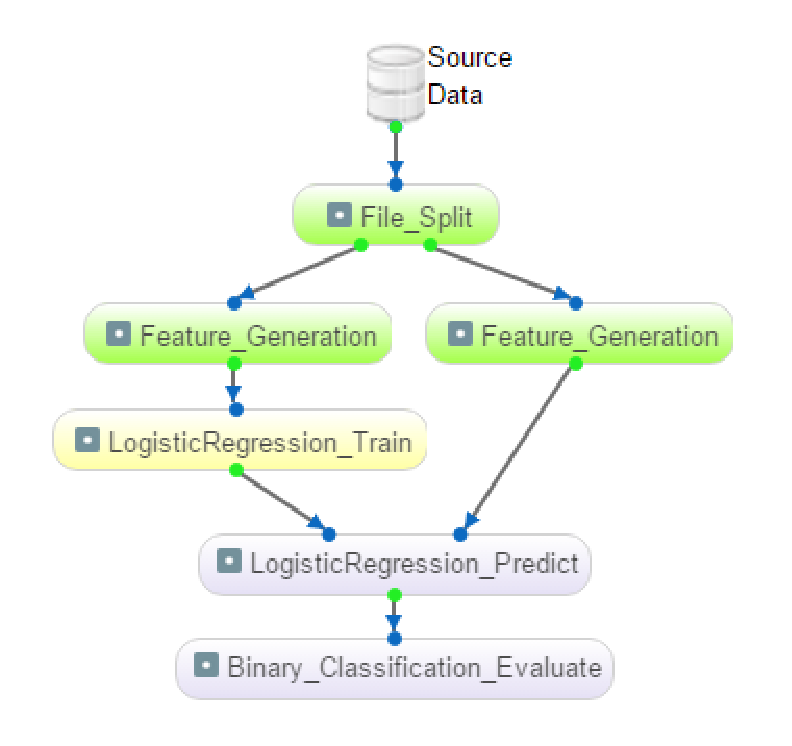
\includegraphics[width = 0.4\textwidth]{LR_DAG.eps}
\caption{An example dataflow DAG for representing the machine learning process.}
\label{fig:dag}
\end{figure}

\section{System Overview}
\subsection{System Architecture}
The demo is a GUI-based machine learning system designed on distributed environments. We have divided the system into two architecture hierarchies. Figure~\ref{fig:arch} is an overview of our system.

\begin{figure}[!htb]
\centering
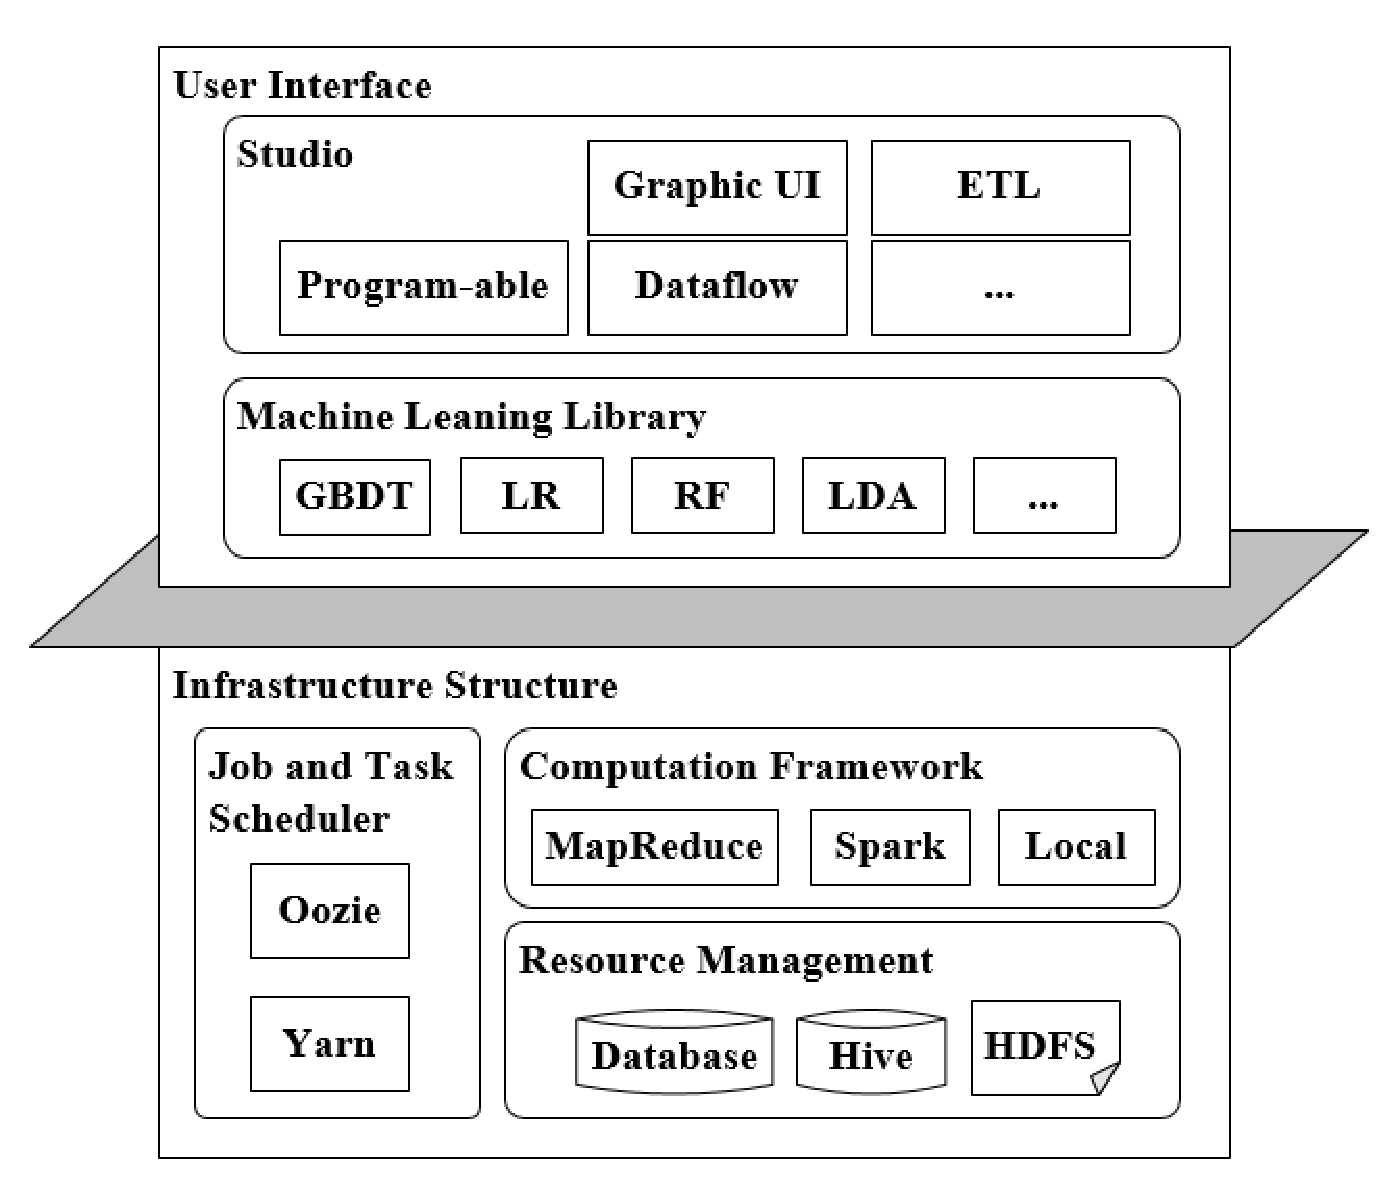
\includegraphics[height=2.5in]{arch.eps}
\caption{An overview of system architecture.}
\label{fig:arch}
\end{figure}

\begin{itemize}
\item \textbf{Layer1:} This is the foundation layer of the system. Oozie is used as job scheduler, where Oozie workflow will be generate according to dataflow DAG. The system support multiple computation frameworks, such as Map-Reduce, Spark and Local. Besides, we use database to store meta data of programs and jobs, while other data resources are stored on HDFS or managed by Hive.
\item \textbf{Layer2:} There are two components in this layer, GUI-based Studio, Machine Learning Library. Studio is in the front end of our system, which provides GUI based dataflow machine learning framework. Machine learning library provide a wealthy of popular algorithms.
\end{itemize}


\subsection{GUI-based Studio}
Studio is a web service in the front end of our system, which allowed user to access to services provided by our system easily. Studio provides functionalities include Graphical UI(GUI), dataflow framework, resource management, and job creation and monitor.

In Studio, datasets and programs are displayed as GUI notes with input/output data ports on the top/bottom. Based on GUI nodes, we implement a GUI based dataflow framework for machine learning job. Under this framework, each GUI node denotes represents an operation( e.g., a machine learning algorithm), and each edge represents the flow of the data from its descendants. 

After a job dataflow DAG is submitted, Studio would generate unique random file path on HDFS for each output port of operation nodes. Then, the job would be sent for scheduling by Oozie and running on Hadoop, where Oozie workflow is generated according dataflow DAG. Based on Oozie, we support job status monitor as well in real time. On the cloud side, each operation is started up by a shell script, which is used to prepare the environment, execute the command line of operation, and do post-processing of the operation.

\subsection{Machine Learning Library}
Machine Learning Library provides a wealth of algorithms, that could be categorized as data pre/post-processing, data format transformation, feature generation, machine learning, and performance evaluation. We have both Standalone and Spark implementations for each algorithm. Also, we provide a sort of API for Machine Learning Lib. 

All these algorithms are wrap as runnable programs and uploaded to our system. The runnable programs uploaded are displayed as GUI nodes of our system that are reusable. In this way, the user is free to program, and enabled to focus on the usage of algorithms. Besides, our system allows registers to upload custom programs and third party programs to our system as well. This is different from traditional tools that are forbidden program upload.

\section{Advantages}
Our system has devoted to provide powerful and light solution for machine learning tasks. And it has many advantages compared to traditional tools, such as enable to process massive data, high scalability and performance etc. Beyond that, we are going to introduce some main advantages of our system.
\subsection{Lowing the Barriers}
A machine learning job is formulated as GUI-based dataflow in our system. Datasets and Programs are displayed as GUI components as well. Users are enabled to create, configure, submit, and monitor a job in drag-and-drop manner. Also, users could track the status of job according to the state reported by dataflow DAG at runtime. The workload of workflow configurations is replaced by drawing dataflow. The implementation details of programs and the diversity of programs are hidden, while the usage are emphasized. Besides, job schema could be save, modify and reuse.

In this way, machine learning is no longer a tough task. Because users are trouble by the complicated implementation and obscure command usage of algorithms no longer. Also, machine learning job construction is fairly easy in drag-and-drop manner. It's easy to understand and create a job in our system even for freshmen.

\subsection{Highly Reusable}
As is shown above, Studio has managed a lot of resources, include dataset, program, job schema, intermediate output data. And we have done effort to make these resources to obtain fully utilized, which is approved to improve our system's user experience.

Reusability is highly supported in different aspects and granularity by our system.  Correspondingly, we have datasets and program reuse, job schema reuse and intermediate output data reuse.

The datasets and programs could be shared across different users, so that one may not need to upload a new program or dataset if there exists one in our system. Although, it is never mind to exists several program for the same algorithm, that gives user more choices and help select out the one better. 

The job schema is a XML document defines the elements, parameters and types that represent a job in our system. With job schema, it is easily to save, modify, reload and reuse a job. When the job finished error or one need to modify the job, it is not necessary to create a job new. One could directly open the old job and modify, then rerun it. Accordingly, the job schema will be update after the job is edited, while the old one be backed. We also support url get request for job, so that one could share and access to a job easily. In addition, jobs are enabled to be clone that greatly facilitate who want to construct several similar jobs.

Intermediate output data is also reuse in our system. The same input and parameters for the same program will generate the same result( without randomness). It's not required to run every time even if the program has random. Therefore, it would reduce running time and save computation and storage greatly with reuse of intermediate output data. We support intermediate output data save and download functions. When a job is modify, we intelligently analysis whether actions in the job should be rerun according to actions' configuration. If the rerun actions will reuse the intermediate output data of non-rerun ones.


\subsection{Heterogeneous System Architecture}

As we all known, machine learning job always consist of several diverse operations. Usually, they might be implemented using variety tools and languages, and run in different manners( Standalone or Distributed, Map-Reduce or Spark etc.) appropriately. 

Fortunately, jobs are regarded as data transformation in dataflow framework. That's job operations are black boxes communicated with data flows. And it's never mind that operations are heterogeneous.

We seamlessly integrated standalone as well as distributed algorithms in one job. All resources are persist on HDFS or managed by Hive in our system. All program will be start up by a start-up script. For standalone program, the script will download the resources demanded for the standalone program before start up it and then upload the result outputs after it finished. For some small dataset, standalone programs might be more time saving and less resource consuming. While, distributed programs have advantages in processing massive data. Hence, with the correct combinations of programs, our system will leverage their advantages.

In our system, each program is running by executed a shell command line in the start-up script. In this way, we support tools of different languages run together, includes C/C++, Java, Scala, python, shell etc, which gives user more unrestrained language choices.

\section{Conclusions}
Machine learning algorithms have become the key components in many cutting edge big data applications. In this demo we present a general-purpose dataflow-based system for easing the process of applying machine learning algorithms to real world tasks. Advantages of the system include 1) lowing the barriers of understanding and applications of machine learning; 2) sharing the implementations of the algorithms, the job DAGs, and re-using the (intermediate) experimental results; 3) seamlessly integrating the stand-alone algorithms as well as the distributed algorithms in one job.

%ACKNOWLEDGMENTS are optional
\section{Acknowledgments}
This section is optional; it is a location for you
to acknowledge grants, funding, editing assistance and
what have you.  In the present case, for example, the
authors would like to thank Gerald Murray of ACM for
his help in codifying this \textit{Author's Guide}
and the \textbf{.cls} and \textbf{.tex} files that it describes.

%APPENDICES are optional
%\balancecolumns
\appendix
%Appendix A

Online system URL is http://159.226.40.104:18080/studio/. 

\textbf{System Home Page}
\begin{figure}[!htb]
\centering

\includegraphics[width = 0.5\textwidth]{HomePage.eps}
\caption{An example dataflow DAG for representing the machine learning process.}
\label{fig:dag}
\end{figure}


\begin{figure}[!htb]
\centering
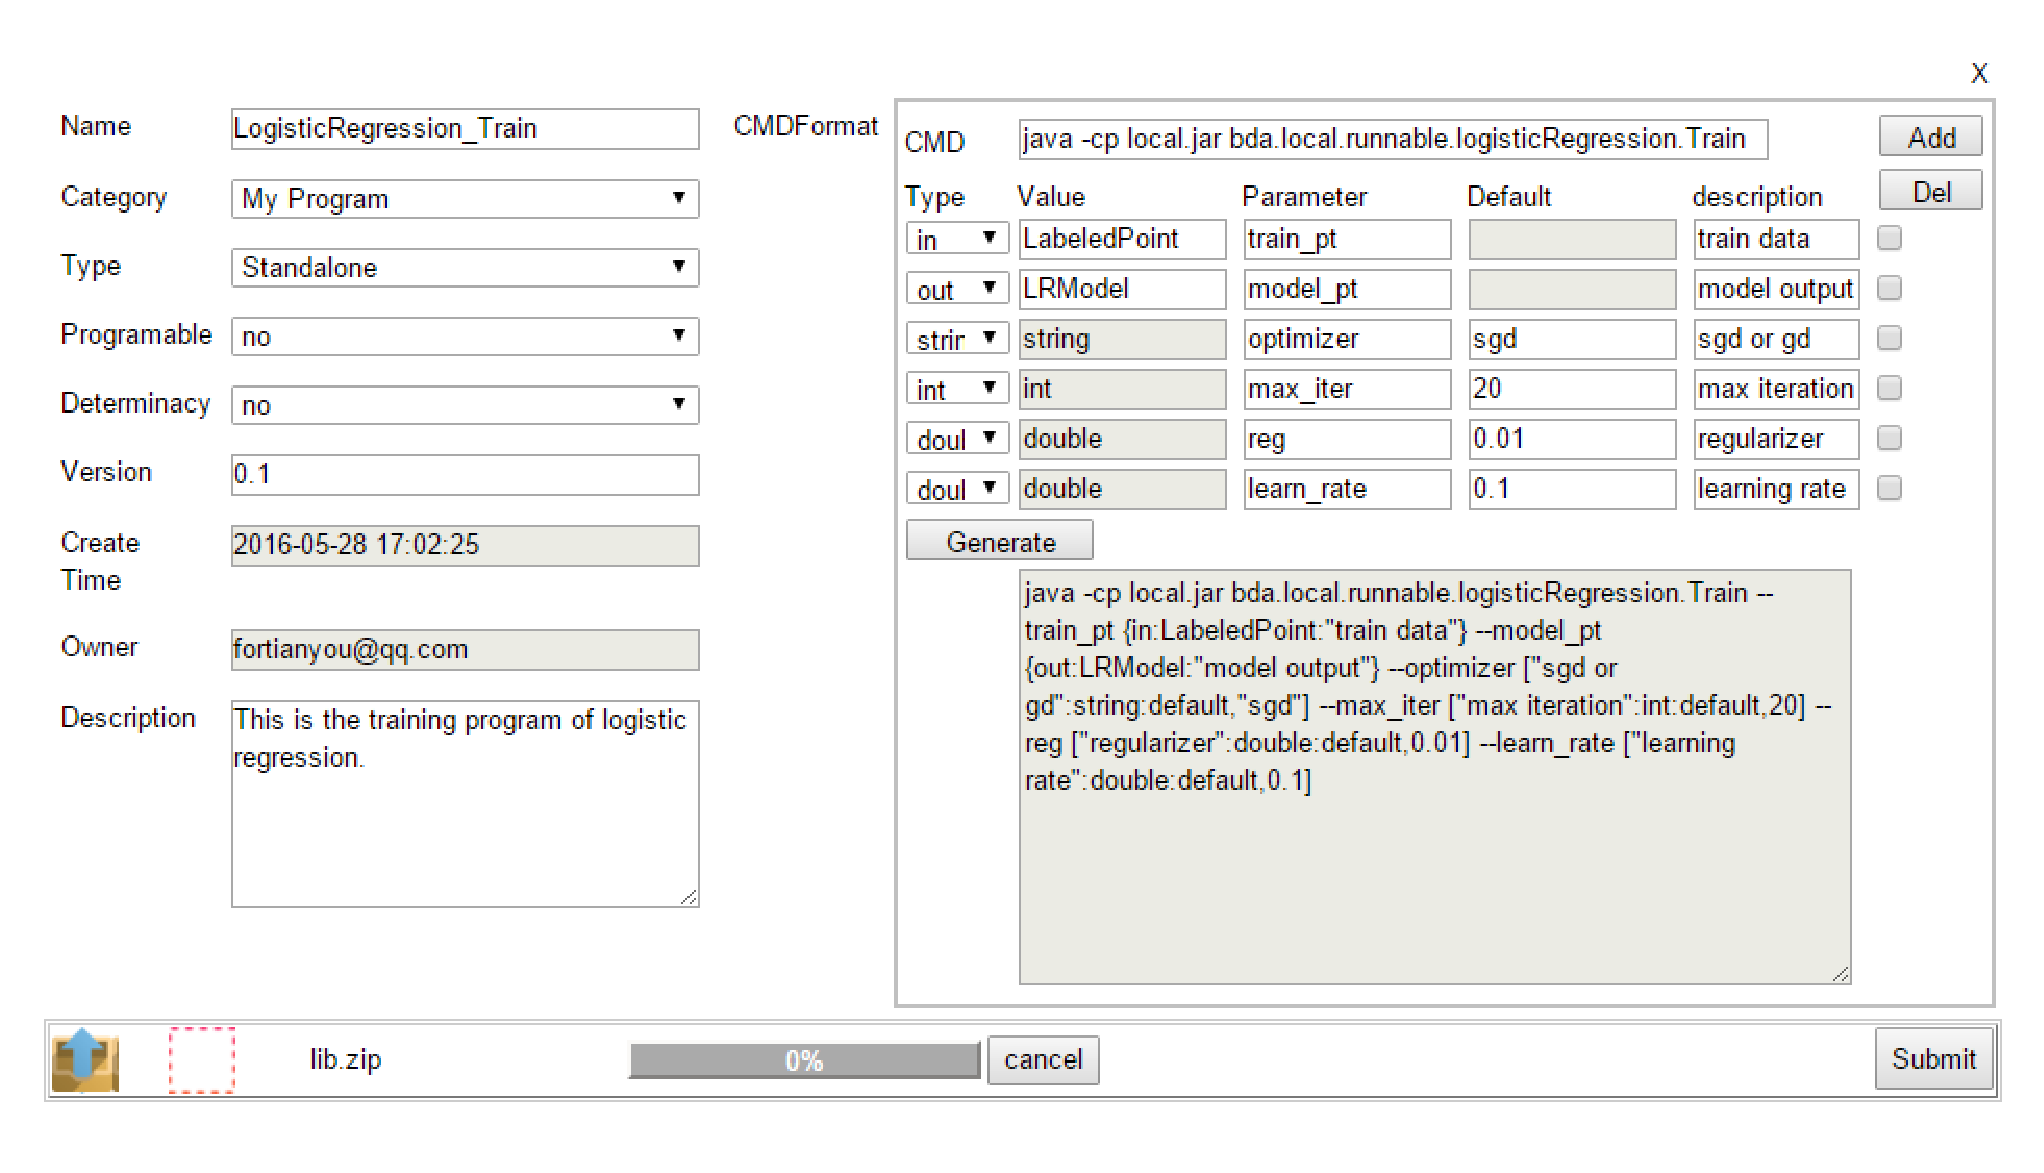
\includegraphics[width = 0.5\textwidth]{Upload_Program.eps}
\caption{An example dataflow DAG for representing the machine learning process.}
\label{fig:dag}
\end{figure}


\begin{figure}[!htb]
\centering
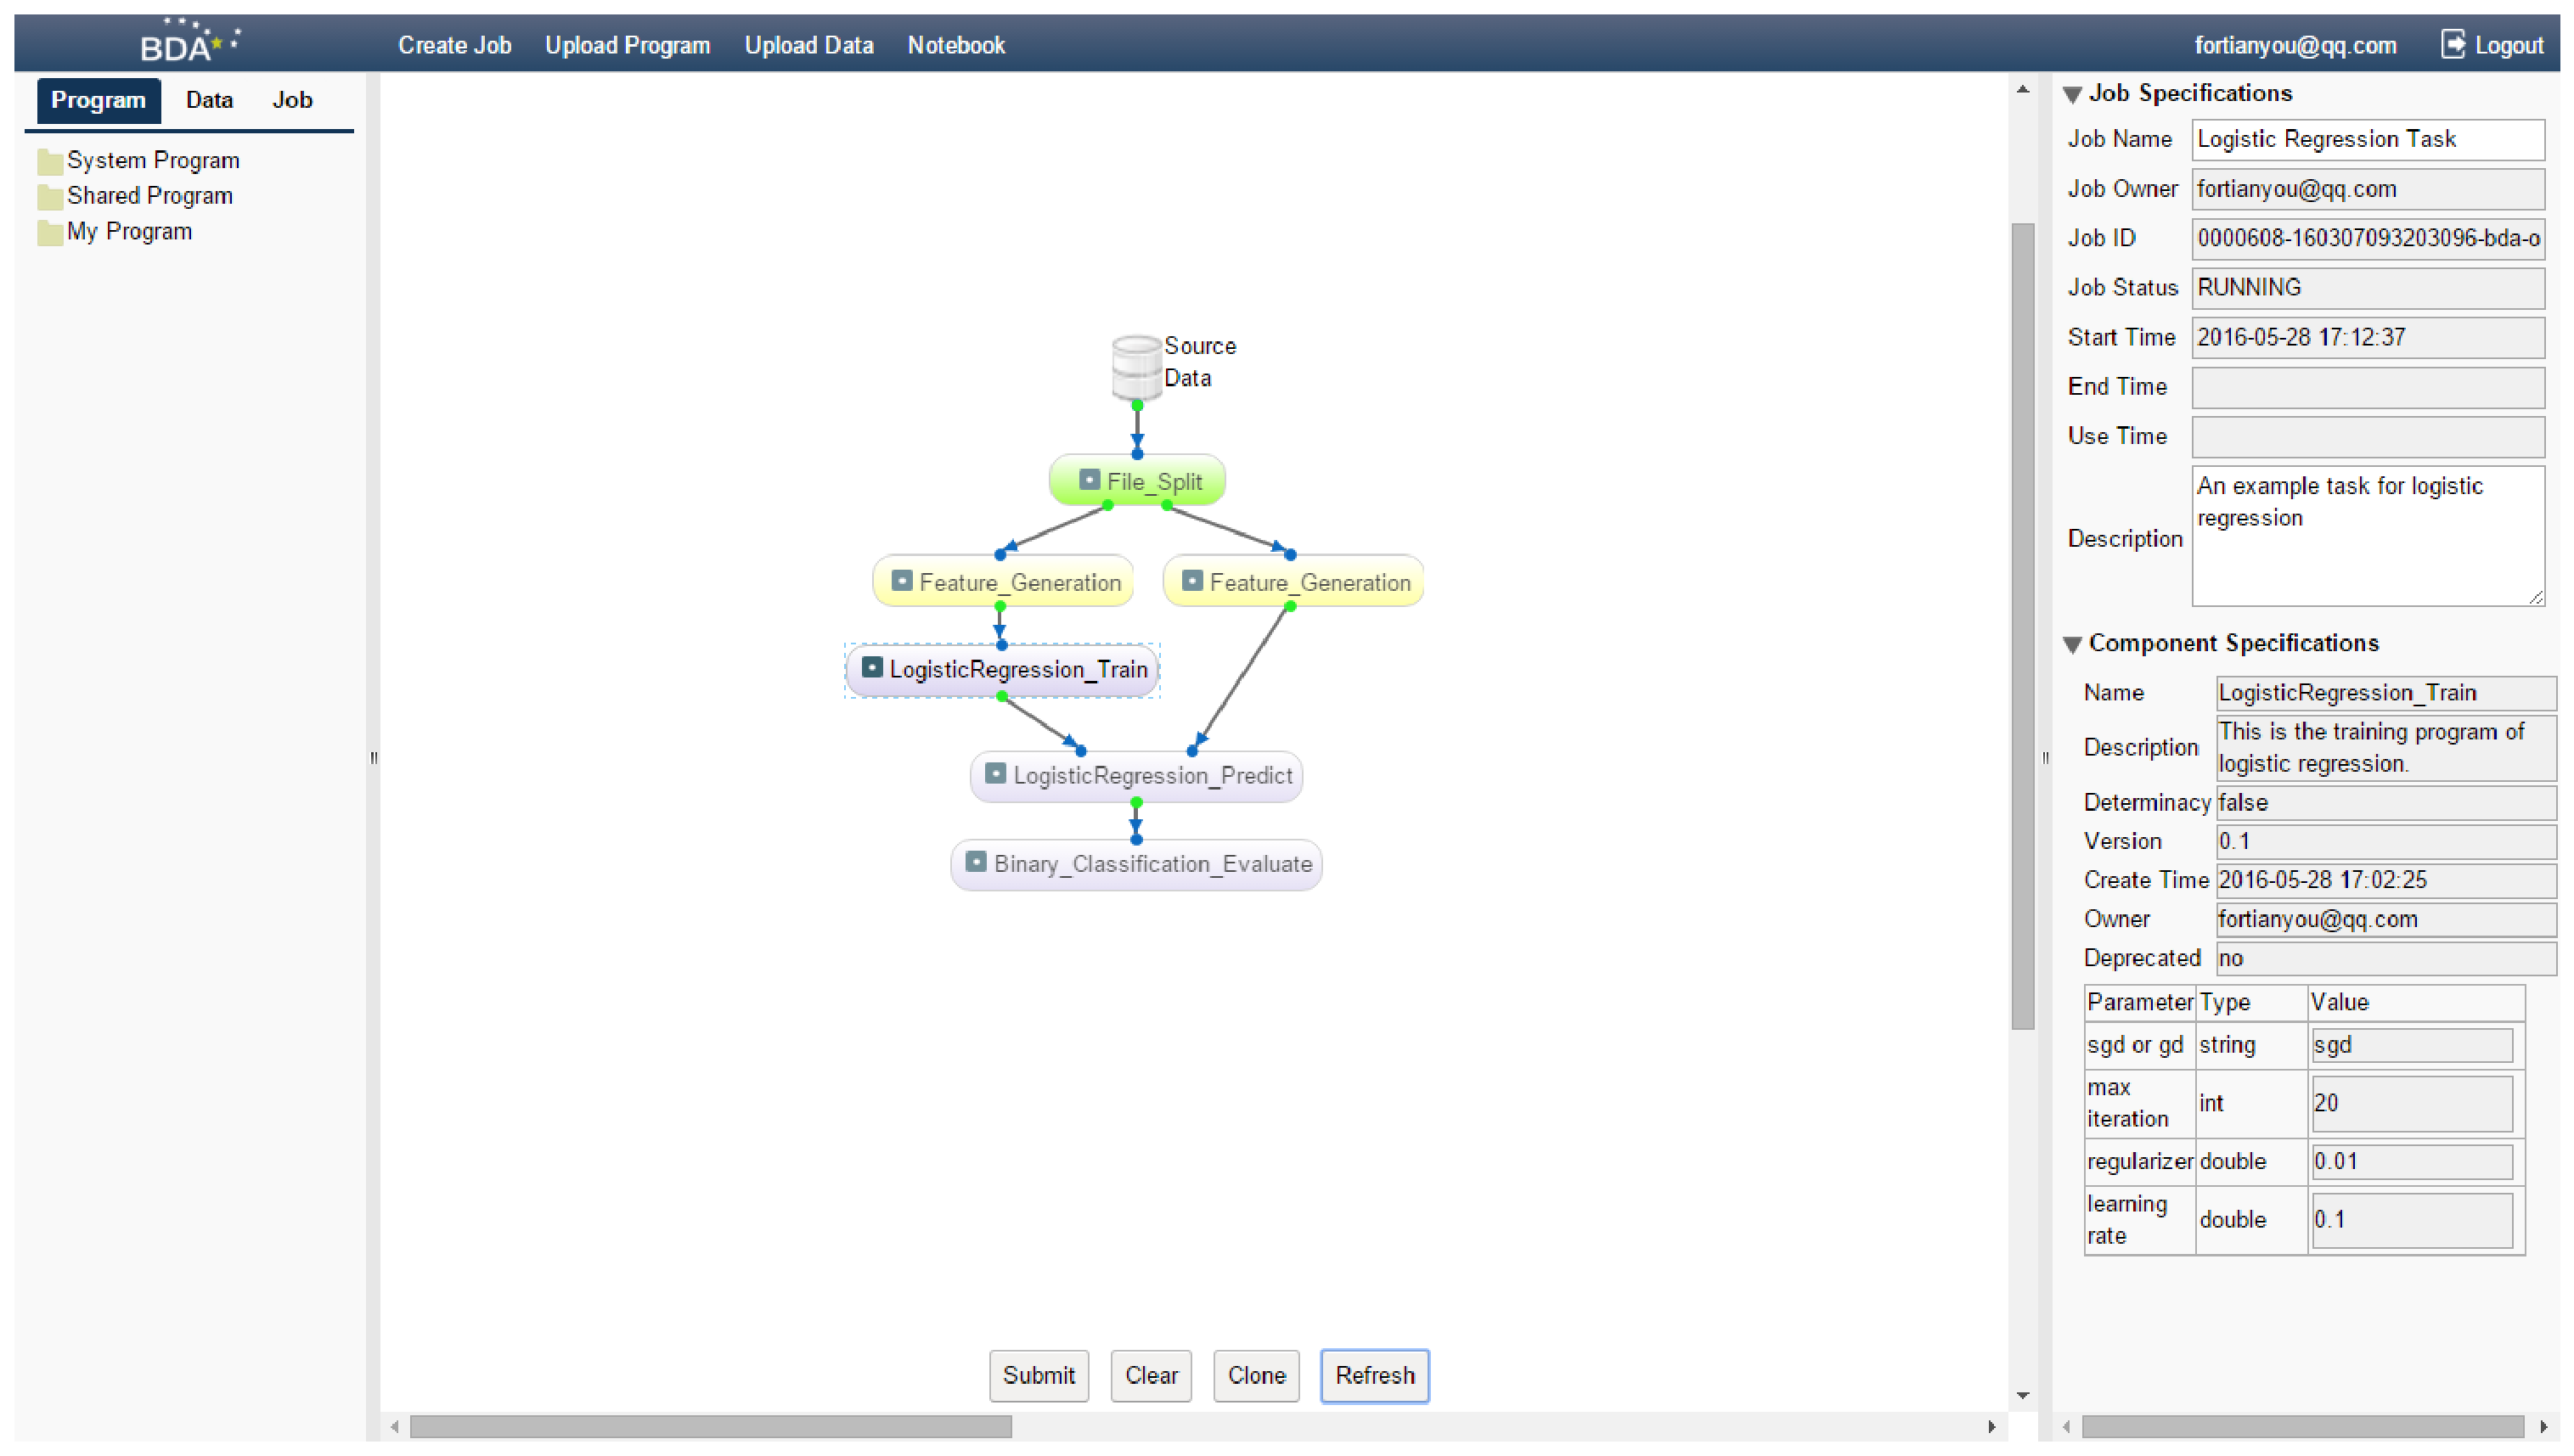
\includegraphics[width = 0.5\textwidth]{LR_Task_example.eps}
\caption{An example dataflow DAG for representing the machine learning process.}
\label{fig:dag}
\end{figure}

\begin{figure}[!htb]
\centering
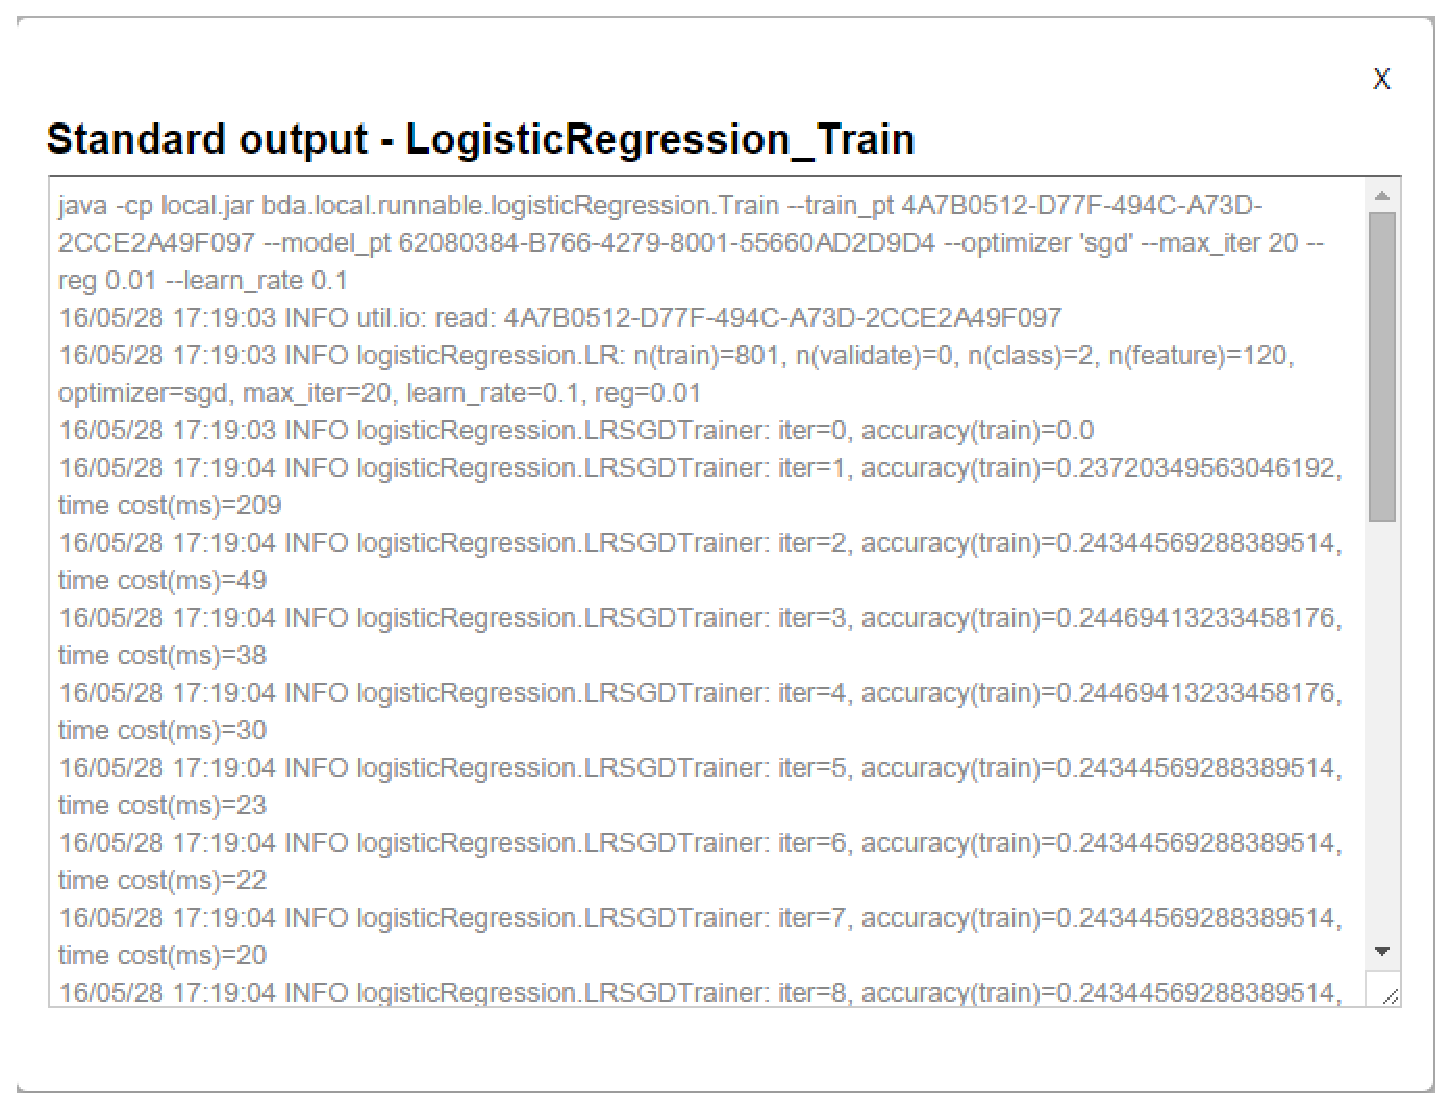
\includegraphics[width = 0.5\textwidth]{LR_Task_stdout.eps}
\caption{An example dataflow DAG for representing the machine learning process.}
\label{fig:dag}
\end{figure}
\end{document}
